\section{Configuration Flow for Option B}
Option A consisted of having the fluids travel in counter-flow configuration with the waste water fluid traveling in the outer tube and the cold water traveling through the inner tube. For Option B however, the fluids remain in the counter-flow setup but the cold water now travels through the outer tube and the waste water is traveling through the inner tube. \\ \\
\noindent
When calculating the outlet temperatures of the hot and cold fluids as the mass flow ratio increased, the plot looked relatively similar. Option A needed to plotted against Option B and a gap between the two data sets can be seen. This can be seen in the figure below and the results show that when the mass flow ratio is below 1, option A is better because the final temperature at the cold water outlet is hotter. However if the mass flow ratio is above 1, option B is greater because the outlet temperature is greater than that of option A. Both options meet the constraint of the outlet of the waste water being 10K higher. Note that the cold mass flowrate is held constant for all cases at 2 kg/s.
%
\begin{figure}[H]
    \label{fig:part_4_1}
    \centering
    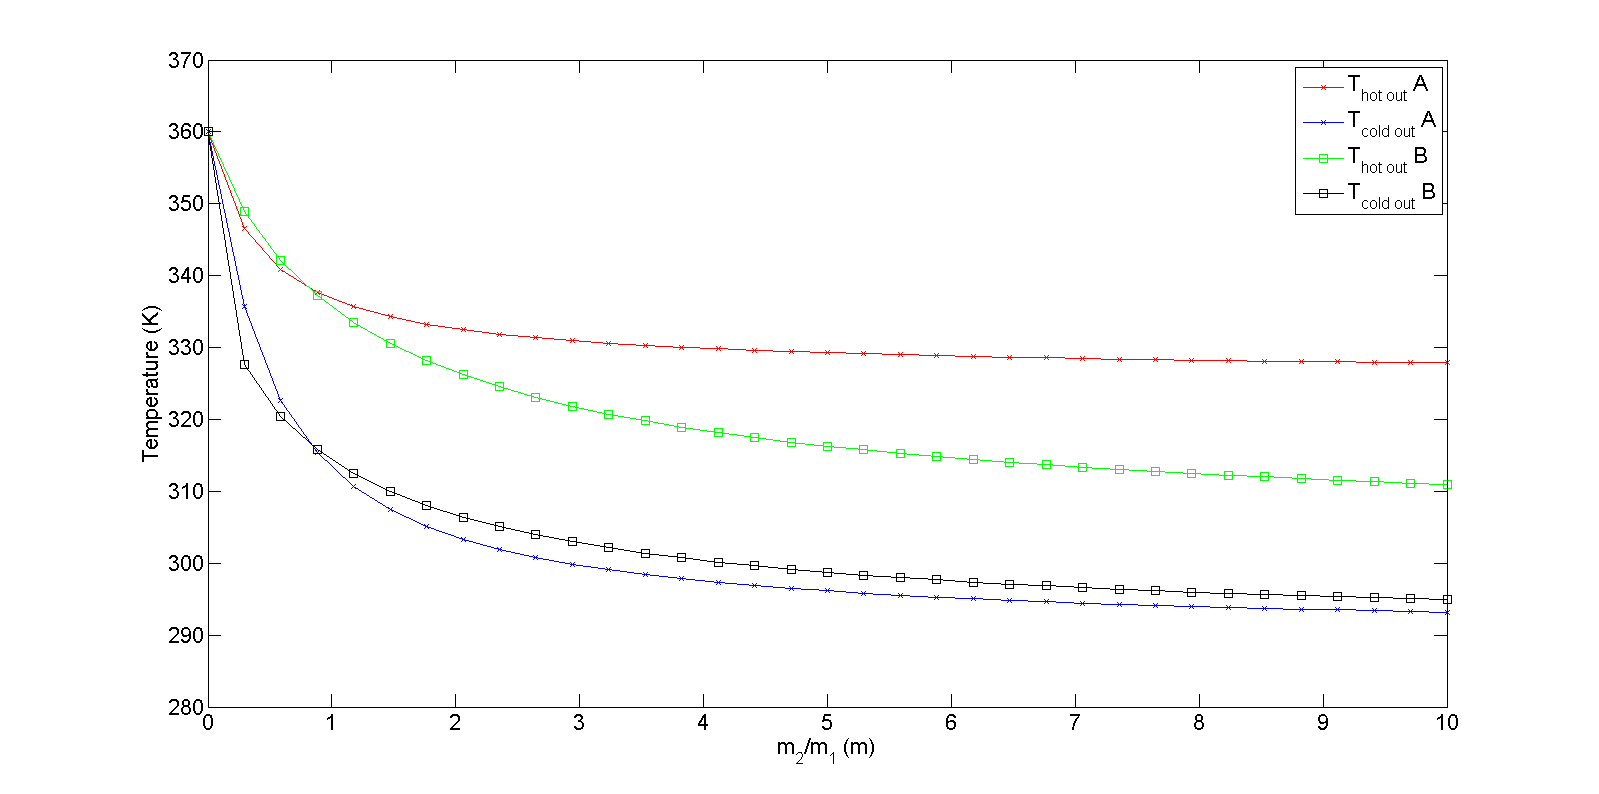
\includegraphics[height=3.5in]{pictures/part_4_temp_vs_massflow.png}
\end{figure}
%
\noindent
To judge the performance of the two systems, one can look at each of their effectiveness. From the figure below, it can be seen that the overall effectiveness of Option B is far greater than that of Option A. The reason for the effectiveness being greater in Option B is that the cold water flow Reynolds number for the outer flow is greater compared to the cold water flow Reynolds number in option A which increases the overall total resistance which in turn reduces the value of the NTU value and increasing the effectiveness. 
%
\begin{figure}[H]
    \centering
    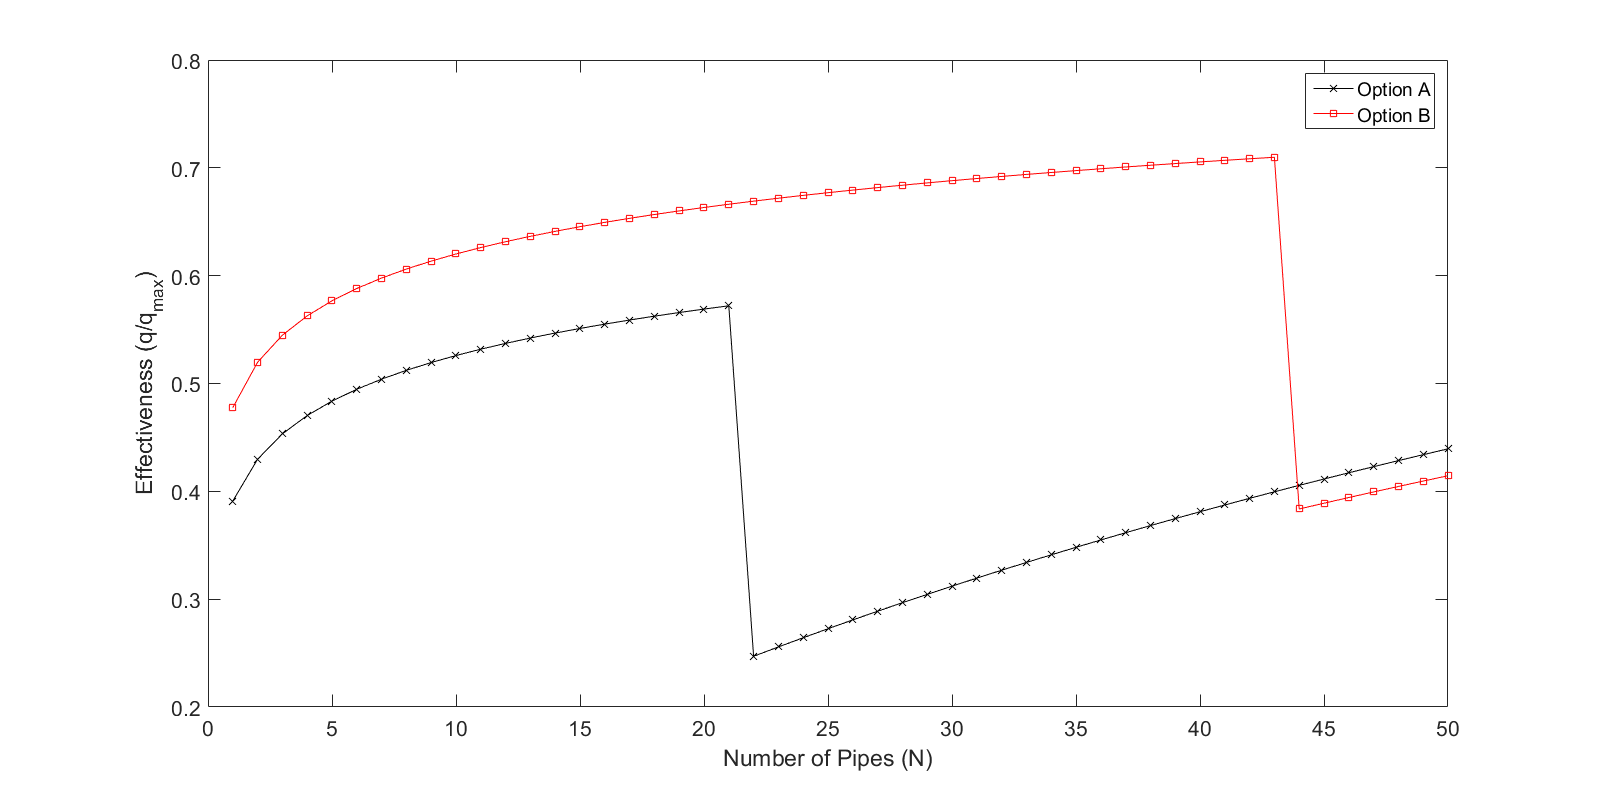
\includegraphics[height=3.5in]{pictures/part_4_eff_050.png}
\end{figure}
%
\noindent
It is interesting to note that their is still the transition to laminar flow of the varying cold mass flowrate. When the cold water is on the outside of the exchanger this happens at a much higher mass flow rate because of the Reynolds number effect described above. It is important to note that when the number of pipes becomes very large we have the hot water transition to a laminar flow. As seen in the figure below this brings the two different configurations to the same performance level when the number of pipes become very large.
%
\begin{figure}[H]
    \centering
    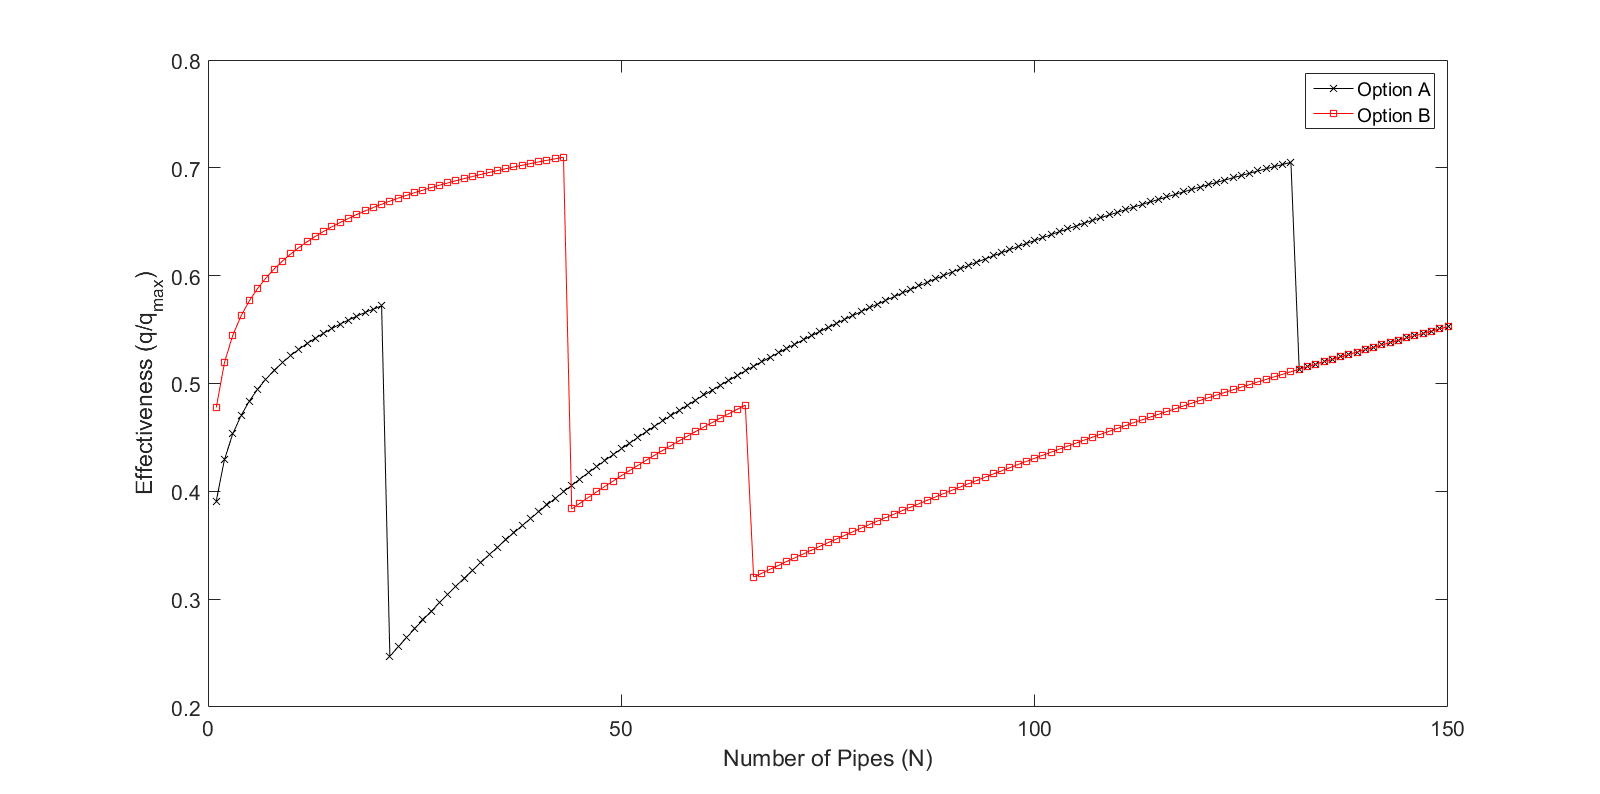
\includegraphics[height=3.5in]{pictures/part_4_eff_150.png}
\end{figure}
%
\noindent
For the final part of analyzing option B, the outlet temperatures needed to be observed with different lengths. To do this the value of the mass flow ratio was a constant value for one iteration and the length varied. This produced the figure seen below just with at different ratios of mass flow rate. It can be deduced that the heat exchanger with larger length tubes and small mass flow ratio produces a hotter cold outlet temperature. Refer to Appendix A for individual graphs of hot water outlet and cold water outlet temperatures. 
%
\begin{figure}[H]
    \centering
    \label{fig_part_4_temps}
    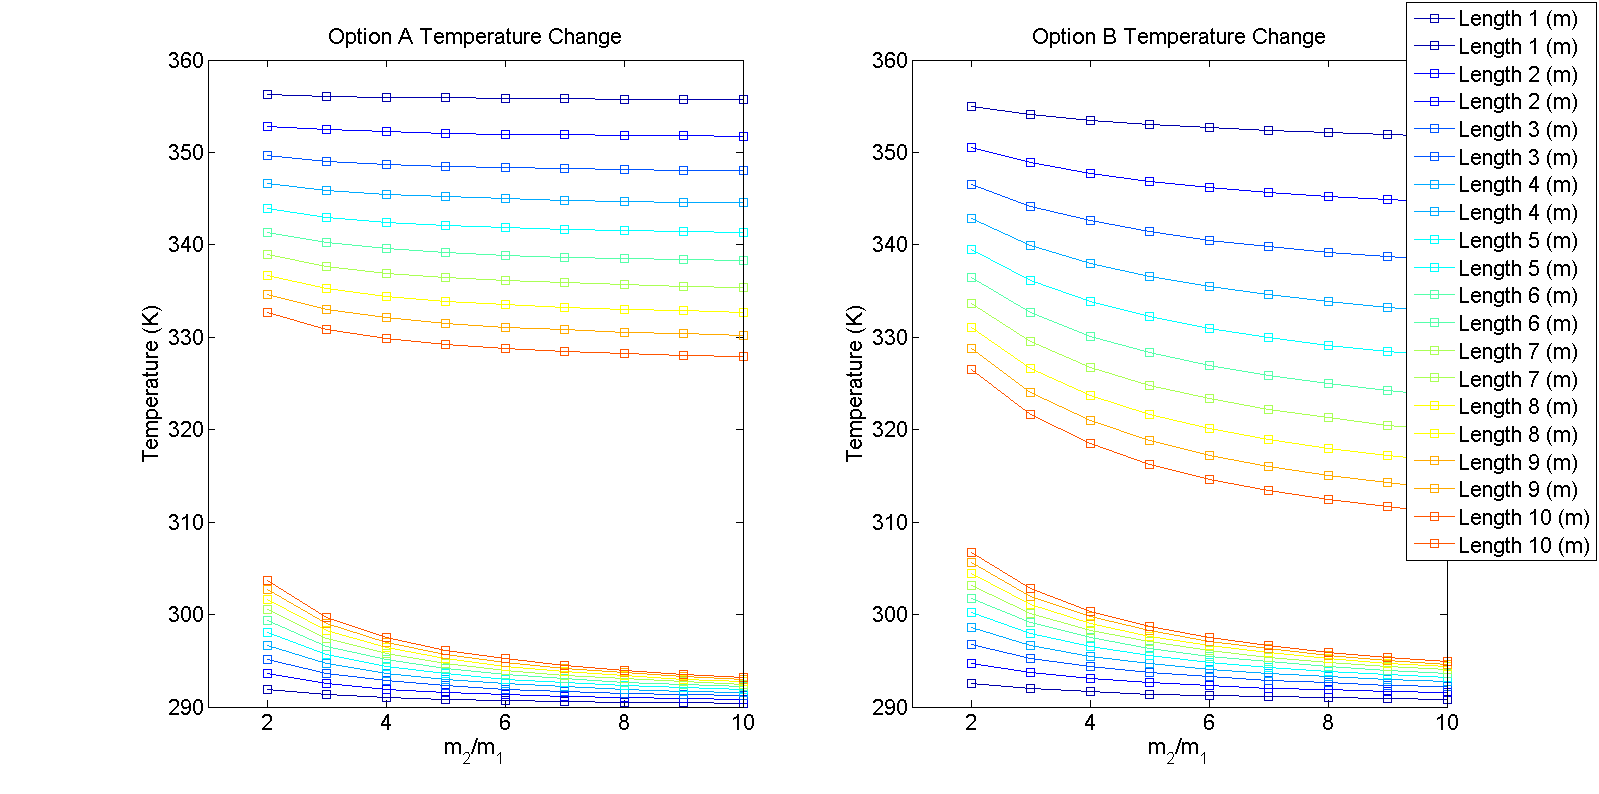
\includegraphics[height=3.5in]{pictures/part_4_total_temp_lengths.png}
\end{figure}
%
\noindent
When analyzing the effectiveness of the heat exchanger as the number of tubes increase at different length values, it can be seen in the figure below that a heat exchanger with the largest length also performs the best with approximately 43 tubes. Although the heat exchanger cannot use more than 8 tubes, option B still outperforms Option A at the greatest length of 10 meters.
%
\begin{figure}[H]
    \centering
    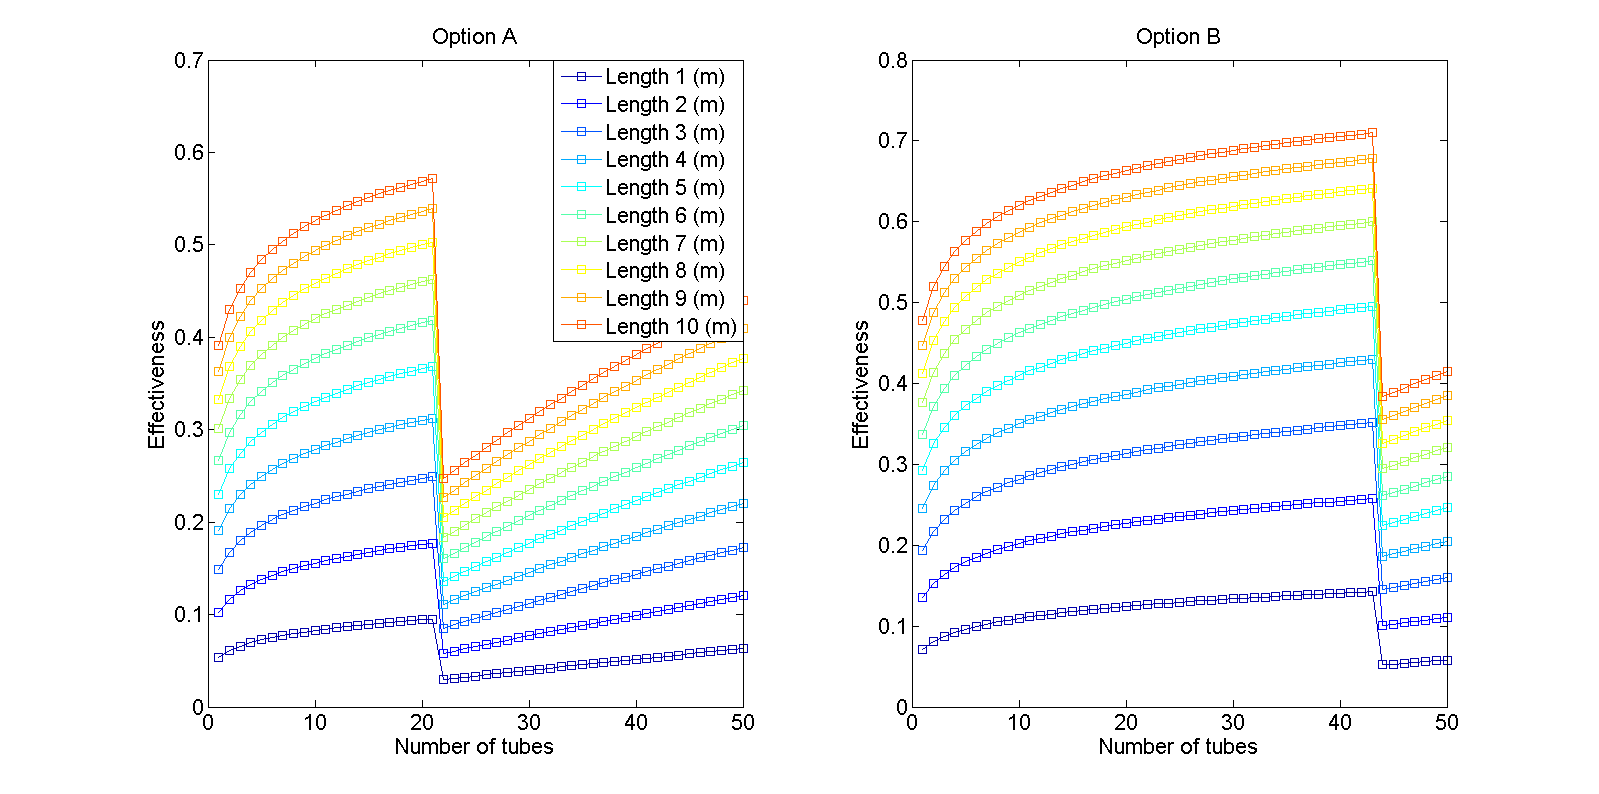
\includegraphics[height=3.5in]{pictures/part_4_tubes_effectiveness_length.png}
\end{figure}
%